\begin{center}
	\begin{tabular}{M{6.5cm}M{11cm}}
		\textbf{LỚP CÔ THẢO - THẦY SANG}& \textbf{ĐỀ ÔN TẬP KIỂM TRA GIỮA HỌC KÌ 1}\\
		\textbf{MÃ ĐỀ: 002}& \textbf{Bài thi môn: VẬT LÝ 11}\\
		\textit{(Đề thi có 06 trang)}& \textit{Thời gian làm bài: 50 phút, không kể thời gian phát đề}
		
		\noindent\rule{4cm}{0.8pt} \\
	\end{tabular}
\end{center}
\setcounter{section}{0}
\section{Câu trắc nghiệm nhiều phương án lựa chọn}
\textit{Thí sinh trả lời từ câu 1 đến câu 18. Mỗi câu hỏi thí sinh chọn một phương án}
\setcounter{ex}{0}
\Opensolutionfile{ans}[ans/G11-5-TN]
% ===================================================================
\begin{ex}
	Khi vật thực hiện một dao động tương ứng với pha dao động sẽ thay đổi một lượng 
	\choice
	{$\SI{0}{\radian}$}
	{$\xsi{\dfrac{\pi}{2}}{\radian}$}
	{$\xsi{\pi}{\radian}$}
	{\True $\xsi{2\pi}{\radian}$}
	\loigiai{}
\end{ex}
% ===================================================================
\begin{ex}
	Đơn vị đo của tần số dao động trong hệ đơn vị SI là 
	\choice
	{\True $\si{\hertz}$}
	{$\si{\second}$}
	{$\si{\centi\meter}$}
	{$\si{\meter}$}
	\loigiai{}
\end{ex}
% ===================================================================
\begin{ex}
	Trong dao động điều hoà, khoảng thời gian mà vật thực hiện được 1 dao động toàn phần gọi là
	\choice
	{biên độ}
	{\True chu kì}
	{tần số}
	{pha ban đầu}
	\loigiai{Khoảng thời gian mà vật thực hiện được 1 dao động toàn phần gọi là chu kì dao động.}
\end{ex}
% ===================================================================
\begin{ex}
	Một bạn học sinh quan sát thấy con lắc trong đồng hồ quả lắc thực hiện được 20 dao động trong 30 giây. Dao động của con lắc trong đồng hồ này có đặc điểm nào sau đây?
	\choice
	{Dao động điều hoà, tần số là $\SI{1.5}{\hertz}$}
	{Dao động điều hoà, tần số là $\SI{0.7}{\hertz}$}
	{Dao động tuần hoàn, tần số là $\SI{1.5}{\hertz}$}
	{\True Dao động tuần hoàn, tần số là $\SI{0.7}{\hertz}$}
	\loigiai{Dao động của con lắc đồng hồ là dao động tuần hoàn với tần số
		$$f=\dfrac{N}{\Delta t}=\dfrac{20}{\SI{30}{\second}}\approx\SI{0.67}{\hertz}.$$}
\end{ex}
% ===================================================================
\begin{ex}
	Một vật dao động điều hoà trên trục $Ox$. Hình bên là đồ thị biểu diễn sự phụ thuộc của li độ $x$ vào thời gian $t$. Tần số góc của dao động là
	\begin{center}
		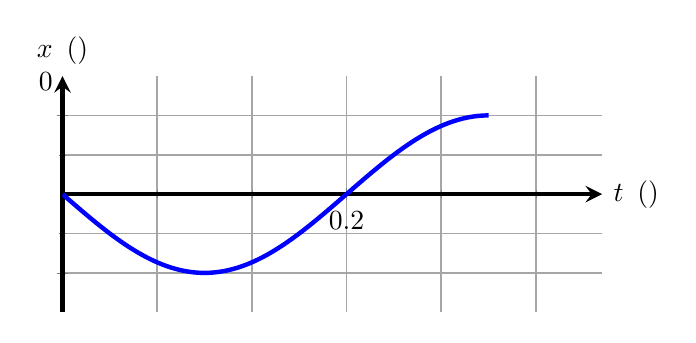
\begin{tikzpicture}  
			\begin{axis}[  ultra thick,
				xmin=0,  
				xmax=0.38,  
				xtick={0,0.2,0.4},
				ytick={-2,0,2},
				minor x tick num=2,
				minor y tick num=1,
				ymin=-3,  
				ymax=3, 
				y=0.5cm,
				samples=300,
				yticklabels=\empty,
				axis lines=center, 
				grid style={step=1, color=gray!70!white, line width=0.6pt},
				grid=both,
				xlabel=$t\ \left(\si{\second}\right)$, 
				ylabel=$x\ \left(\si{\centi\meter}\right)$, 
				every axis y label/.style={at=(current axis.above origin),anchor=south},  
				every axis x label/.style={at=(current axis.right of origin),anchor=west},  ]
				\addplot [ultra thick, blue, smooth, domain=0:0.3] {2*cos(deg(5*pi*x+pi/2))}; 
			\end{axis}  
			\node[label={[left]90:0}] at (0,2.8){};
		\end{tikzpicture}
	\end{center}
	\choice
	{$\SI{10}{\radian/\second}$}
	{$\xsi{10\pi}{\radian/\second}$}
	{\True $\xsi{5\pi}{\radian/\second}$}
	{$\SI{5}{\radian/\second}$}
	\loigiai{Chu kì dao động của vật $T=\SI{0.4}{\second}$.\\
		Tần số góc dao động:
		$$\omega=\dfrac{2\pi}{T}=\xsi{5\pi}{\radian/\second}.$$}
\end{ex}
% ===================================================================
\begin{ex}
	Các nhà thực nghiệm đo được tần số dao động của một hệ gồm thanh silicon siêu nhỏ có virus dính trên đó đang thực hiện dao động là $\SI{2.87E14}{\hertz}$. Tần số góc của hệ dao động trên bằng bao nhiêu? 
	\choice
	{\True $\SI{1.80E15}{\radian/\second}$}
	{$\SI{3.48E15}{\radian/\second}$}
	{$\SI{2.18E14}{\radian/\second}$}
	{$\SI{4.57E14}{\radian/\second}$}
	\loigiai{Tần số góc của dao động:
		$$\omega=2\pi f=\SI{1.80E15}{\radian/\second}.$$}
\end{ex}
% ===================================================================
\begin{ex}
Một con lắc là xo gồm vật nhỏ và lò xo nhẹ có độ cứng $k$, đang dao động điều hòa. Mốc thế năng tại vị trí cân bằng. Biểu thức thế năng của con lắc ở li độ $x$ là
	\choice
	{$2kx$}
	{\True $\dfrac{kx^2}{2}$}
	{$2kx^2$}
	{$\dfrac{kx}{2}$}
	\loigiai{}
\end{ex}
% ===================================================================
\begin{ex}
	Khi nói về dao động điều hòa của một vật, phát biểu nào sau đây \textbf{đúng}?
	\choice
	{Khi vật ở vị trí biên, gia tốc của vật bằng không}
	{\True Vectơ gia tốc của vật luôn hướng về vị trí cân bằng}
	{Vectơ vận tốc của vật luôn hướng về vị trí cân bằng}
	{Khi đi qua vị trí cân bằng, vận tốc của vật bằng không}
	\loigiai{}
\end{ex}
% ===================================================================
\begin{ex}
Khi tiến hành thí nghiệm khảo sát vị trí vật nặng của con lắc lò xo đang dao động bằng cách sử dụng thước thẳng, bạn học sinh thấy rằng vật nặng dao động từ vị trí $\SI{1}{\centi\meter}$ đến vị trí $\SI{11}{\centi\meter}$ trên thước. Biên độ dao động của vật nặng trong con lắc lò xo là	
	\choice
	{$\SI{10}{\centi\meter}$}
	{$\SI{6}{\centi\meter}$}
	{\True $\SI{5}{\centi\meter}$}
	{$\SI{12}{\centi\meter}$}
	\loigiai{Biên độ dao động của vật nặng trong con lắc lò xo:
		$$A=\dfrac{\ell_\text{max}-\ell_\text{min}}{2}=\SI{5}{\centi\meter}.$$}
\end{ex}
% ===================================================================
\begin{ex}
	Hai vật dao động điều hoà có đồ thị li độ - thời gian như hình vẽ. Phát biểu nào sau đây mô tả đúng tính chất của hai vật?
	\begin{center}
		\includegraphics[width=0.6\linewidth]{../figs/D11-2-1}
	\end{center}
	\choice
	{Hai vật dao động cùng tần số, cùng pha}
	{\True Hai vật dao động cùng tần số, vuông pha}
	{Hai vật dao động khác tần số, cùng pha}
	{Hai vật dao động khác tần số, vuông pha}
	\loigiai{Dựa vào đồ thị li độ - thời gian, ta nhận thấy hai vật dao động cùng tần số.\\
		Tại thời điểm $t=0$, vật 2 qua VTCB theo chiều dương. Sau khoảng thời gian $\Delta t=\dfrac{T}{4}$ vật 1 có cùng trạng thái dao động với vật 2 ở thời điểm $t=0$. Suy ra, độ lệch pha giữa hai dao động:
		$$\Delta \varphi=\dfrac{\Delta t}{T}\cdot2\pi=\xsi{\dfrac{\pi}{2}}{\radian}.$$}
\end{ex}
% ===================================================================
\begin{ex}
Đồ thị li độ thời gian của một vật dao động điều hoà được thể hiện như hình vẽ. Phương trình dao động của vật là
\begin{center}
	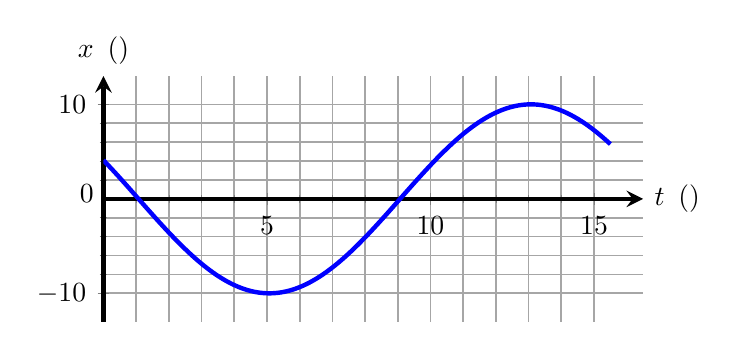
\begin{tikzpicture}  
		\begin{axis}[  ultra thick,
			xmin=0,  
			xmax=16.5,  
			xtick={0,5,10,15},
			ytick={-10,0,10},
			minor x tick num=4,
			minor y tick num=4,
			ymin=-13,  
			ymax=13, 
			y=0.12cm,
			samples=300,
			axis lines=center, 
			grid style={step=1, color=gray!70!white, line width=0.6pt},
			grid=both,
			xlabel=$t\ \left(\si{\second}\right)$, 
			ylabel=$x\ \left(\si{\centi\meter}\right)$, 
			every axis y label/.style={at=(current axis.above origin),anchor=south},  
			every axis x label/.style={at=(current axis.right of origin),anchor=west},  ]
			\addplot [ultra thick, blue, smooth, domain=0:15.5] {10*cos(deg(pi*x/8+1.15))}; 
		\end{axis}  
		\node[label={[left]90:0}] at (0,1.5){};
	\end{tikzpicture}
\end{center}	
	\choice
	{$x=\xsi{10\cos\left(16t+1,37\right)}{\centi\meter}$}
	{$x=\xsi{10\cos\left(\dfrac{\pi}{8}t-1,18\right)}{\centi\meter}$}
	{$x=\xsi{10\cos\left(16t-1,37\right)}{\centi\meter}$}
	{\True $x=\xsi{10\cos\left(\dfrac{\pi}{8}t+1,18\right)}{\centi\meter}$}
	\loigiai{Chu kì dao động của vật:
		$$\dfrac{T}{2}=\SI{13}{\second}-\SI{5}{\second}\Rightarrow T=\SI{16}{\second}$$
		Tần số góc dao động:
		$$\omega=\dfrac{2\pi}{T}=\xsi{\dfrac{\pi}{8}}{\radian/\second}$$
		Tại thời điểm $t=\SI{5}{\second}$, vật đang ở vị trí biên âm, pha dao động của vật lúc này
		$$\varphi=\omega t+\varphi_0=\xsi{\pi}{\radian}\Rightarrow \varphi_0=\varphi-\omega t=\xsi{\pi}{\radian}-\left(\xsi{\dfrac{\pi}{8}}{\radian/\second}\right)\cdot\left(\SI{5}{\second}\right)=\xsi{\dfrac{3\pi}{8}}{\radian}\approx\SI{1.18}{\radian}.$$
		Phương trình dao động của vật:
		$$x=\xsi{10\cos\left(\dfrac{\pi}{8}t+1,18\right)}{\centi\meter}.$$}
\end{ex}
% ===================================================================
\begin{ex}
	Một vật dao động điều hoà với chu kì $\SI{2}{\second}$, biên độ $\SI{10}{\centi\meter}$. Khi vật cách vị trí biên $\SI{4}{\centi\meter}$ thì tốc độ của nó bằng
	\choice
	{$\SI{18.33}{\centi\meter/\second}$}
	{$\SI{28.79}{\centi\meter/\second}$}
	{\True $\SI{25.13}{\centi\meter/\second}$}
	{$\SI{18.84}{\centi\meter/\second}$}
	\loigiai{Tốc độ của vật khi cách vị trí biên $\SI{4}{\centi\meter}$ $\left(\left|x\right|=\SI{6}{\centi\meter}\right)$:
		$$\left|v\right|=\omega\sqrt{A^2-x^2}=\left(\dfrac{\xsi{2\pi}{\radian}}{\SI{2}{\second}}\right)\sqrt{\left(\SI{10}{\centi\meter}\right)^2-\left(\SI{6}{\centi\meter}\right)^2}\approx\SI{25.13}{\centi\meter/\second}.$$}
\end{ex}
% ===================================================================
\begin{ex}
	Một vật dao động điều hoà có gia tốc biến đổi theo thời gian $a=\xsi{8\cos\left(20t-\dfrac{\pi}{2}\right)}{\centi\meter/\second^2}$. Phương trình dao động của vật là
	\choice
	{\True $x=\xsi{0,02\cos\left(20t+\dfrac{\pi}{2}\right)}{\centi\meter}$}
	{$x=\xsi{2\cos\left(20t-\dfrac{\pi}{2}\right)}{\centi\meter}$}
	{$x=\xsi{4\cos\left(20t+\dfrac{\pi}{2}\right)}{\centi\meter}$}
	{$x=\xsi{2\cos\left(20t+\dfrac{\pi}{2}\right)}{\centi\meter}$}
	\loigiai{Biên độ dao động của vật:
		$$A=\dfrac{a_\text{max}}{\omega^2}=\dfrac{\SI{8}{\centi\meter/\second^2}}{\left(\SI{20}{\radian/\second}\right)^2}=\SI{0.02}{\centi\meter}$$
		Pha ban đầu của dao động:
		$$\varphi_{0x}=\varphi_{0a}+\pi=\xsi{\dfrac{\pi}{2}}{\radian}.$$
		Vậy phương trình dao động của vật $x=\xsi{0,02\cos\left(20t+\dfrac{\pi}{2}\right)}{\centi\meter}$.}
\end{ex}
% ===================================================================
\begin{ex}
	Một chất điểm dao động điều hoà, gia tốc $a$ và li độ $x$ của chất điểm liên hệ với nhau bởi hệ thức $a=-4\pi^2x$, trong đó $a$ có đơn vị $\si{\centi\meter/\second^2}$; $x$ có đơn vị $\si{\centi\meter}$. Chu kì dao động bằng
	\choice
	{\True $\SI{1}{\second}$}
	{$\SI{0.25}{\second}$}
	{$\SI{0.5}{\second}$}
	{$\SI{0.4}{\second}$}
	\loigiai{Mối liên hệ giữa gia tốc và li độ của vật dao động điều hoà:
		$$a=-\omega^2x\Rightarrow \omega=\xsi{2\pi}{\radian/\second}$$
		$$\Rightarrow T=\dfrac{2\pi}{\omega}=\SI{1}{\second}.$$}
\end{ex}
% ===================================================================
\begin{ex}
Một vật dao động điều hoà trên trục $Ox$ với phương trình $x=\xsi{5\cos\left(4\pi t-\dfrac{\pi}{3}\right)}{\centi\meter}$. Khoảng thời gian ngắn nhất để vật đi từ li độ $x_1=\SI{-2.5}{\centi\meter}$ đến vị trí $x_2=\xsi{\dfrac{5\sqrt{3}}{2}}{\centi\meter}$ là	
	\choice
	{$\xsi{\dfrac{5}{48}}{\second}$}
	{$\xsi{\dfrac{5}{24}}{\second}$}
	{\True $\xsi{\dfrac{1}{8}}{\second}$}
	{$\xsi{\dfrac{3}{20}}{\second}$}
	\loigiai{\begin{center}
			\begin{tikzpicture}
				\coordinate (O) at (0,0);
				\coordinate (A) at (240:3);
				\coordinate (B) at (330:3);
				\coordinate (D) at (5,0);
				\coordinate (E) at (-4,0);
				\draw[line width=1.0] (O) circle[radius=3];
				
				\draw [fill=cyan!20](330:3)--(0,0)--(240:3) arc (240:330:3)--cycle;
				\draw[-stealth, line width=1.0] (E) -- (D);
				\draw[-stealth, line width=1.0] (0,-4) -- (0,4);
				\tkzMarkRightAngle[size=0.3,color=blue](A,O,B);
				\draw[-stealth,thick,red] (O) -- (A);
				\draw[-stealth,thick,red] (O) -- (B);
				\draw[dashed] (A) -- ($(O)!(A)!(D)$);
				\draw[dashed] (B) -- ($(O)!(B)!(D)$);
				
				\fill   (O) circle[radius=2pt]  node [above left] {$O$};
				\fill   ($(O)!(A)!(D)$) circle[radius=2pt, color=teal];
				\fill   ($(O)!(B)!(E)$) circle[radius=2pt,color=teal];
				\fill   (3,0) circle[radius=2pt]  node [above right] {$5$};
				\fill   (-3,0) circle[radius=2pt]  node [above left] {$-5$};
				\node[label={[above]90:$x \left(\si{\centi\meter}\right)$}] at ($(D)-(0,0.2)$){};
				\node[label={[above]90:$-2,5$}] at ($(O)!(A)!(D)$){};
				\node[label={[above left]90:$\dfrac{5\sqrt{3}}{2}$}] at ($(O)!(B)!(D)$){};
			\end{tikzpicture}
		\end{center}
		Dựa vào vòng tròn lượng giác, thời gian ngắn nhất để vật đi từ vị trí $x_1=\SI{-2.5}{\centi\meter}$ đến vị trí $x_2=\xsi{\dfrac{5\sqrt{3}}{2}}{\centi\meter}$
		là
		$$\Delta t=\dfrac{T}{4}=\dfrac{1}{4}\cdot\dfrac{2\pi}{\omega}=\xsi{\dfrac{1}{8}}{\second}
		.$$}
\end{ex}
% ===================================================================
\begin{ex}
	Một vật dao động điều hoà trên quỹ đạo dài $\SI{8}{\centi\meter}$. Tốc độ của vật khi qua vị trí cân bằng là $\xsi{0,4\pi}{\meter/\second}$. Gọi mốc thời gian là lúc vật đi qua vị trí $\xsi{2\sqrt{3}}{\centi\meter}$ theo chiều dương. Phương trình dao động của vật là
	\choice
	{\True $x=\xsi{4\cos\left(10\pi t-\dfrac{\pi}{6}\right)}{\centi\meter}$}
	{$x=\xsi{4\cos\left(10\pi t+\dfrac{\pi}{6}\right)}{\centi\meter}$}
	{$x=\xsi{2\cos\left(10\pi t-\dfrac{\pi}{6}\right)}{\centi\meter}$}
	{$x=\xsi{2\cos\left(10\pi t+\dfrac{\pi}{6}\right)}{\centi\meter}$}
	\loigiai{Biên độ dao động của vật
		$$A=\dfrac{L}{2}=\SI{4}{\centi\meter}$$
		Tần số góc dao động
		$$\omega=\dfrac{v_\text{max}}{A}=\dfrac{\xsi{40\pi}{\radian/\second}}{\SI{4}{\centi\meter}}=\xsi{10\pi}{\radian/\second}$$
		Chọn mốc thời gian lúc vật đi qua vị trí $\xsi{2\sqrt{3}}{\centi\meter}$ theo chiều dương. Pha ban đầu
		$$\varphi_0=-\arccos\dfrac{x_0}{A}=-\xsi{\dfrac{\pi}{6}}{\radian}$$}
\end{ex}
% ===================================================================
\begin{ex}
	Một vật dao động điều hoà trên trục $Ox$. Khi vật qua vị trí cân bằng thì tốc độ của nó là $\SI{20}{\centi\meter/\second}$. Khi vật có tốc độ là $\SI{10}{\centi\meter/\second}$ thì gia tốc của nó có độ lớn $\xsi{40\sqrt{3}}{\centi\meter/\second^2}$. Biên độ dao động của vật bằng
	\choice
	{$\SI{4}{\centi\meter}$}
	{\True $\SI{5}{\centi\meter}$}
	{$\SI{16}{\centi\meter}$}
	{$\SI{8}{\centi\meter}$}
	\loigiai{$$\dfrac{v^2}{v^2_\text{max}}+\dfrac{a^2}{a^2_\text{max}}=1\Rightarrow a_\text{max}=\SI{80}{\centi\meter/\second^2}$$
		Biên độ dao động của vật:
		$$A=\dfrac{v^2_\text{max}}{a_\text{max}}=\SI{5}{\centi\meter}.$$}
\end{ex}
% ===================================================================
\begin{ex}
	Đồ thị động năng theo thời gian của một vật có khối lượng $\SI{0.4}{\kilogram}$ dao động điều hoà. Tại thời điểm ban đầu vật đang chuyển động theo chiều dương. Lấy $\pi^2=10$. Phương trình dao động của vật có dạng
	\begin{center}
		\begin{tikzpicture}  
			\begin{axis}[  ultra thick,
				xmin=0,  
				xmax=1.2,  
				xtick={0,1.0},
				ytick={0,2},
				minor x tick num=5,
				minor y tick num=3,
				yticklabels=\empty,
				xticklabels=\empty,
				ymin=0,  
				ymax=2.5, 
				y=1.5cm,
				samples=300,
				axis lines=center, 
				grid style={step=1, color=gray!70!white, line width=0.6pt},
				grid=both,
				xlabel=$t\ \left(\si{\second}\right)$, 
				ylabel=$W_\text{đ}\ \left(\si{\joule}\right)$, 
				every axis y label/.style={at=(current axis.above origin),anchor=south},  
				every axis x label/.style={at=(current axis.right of origin),anchor=west},  ]
				\addplot [ultra thick, blue, smooth, domain=0:1.0] {1+1*cos(deg(4*pi*x+pi/3))}; 
			\end{axis}  
			\node[label={[left]90:0}] at (0,0){};
			\node[label={[left]90:0,02}] at (0,2.9){};
			\node[label={[below]90:$\dfrac{1}{6}$}] at (1,-0.1){};
		\end{tikzpicture}
	\end{center}
	\choice
	{$x=\xsi{5\cos\left(2\pi t+\dfrac{\pi}{3}\right)}{\centi\meter}$}
	{$x=\xsi{10\cos\left(2\pi t+\dfrac{5\pi}{6}\right)}{\centi\meter}$}
	{$x=\xsi{10\cos\left(2\pi t-\dfrac{5\pi}{6}\right)}{\centi\meter}$}
	{\True $x=\xsi{5\cos\left(2\pi t-\dfrac{\pi}{3}\right)}{\centi\meter}$}
	\loigiai{Chu kì dao động của động năng:
		$$2T'=6\cdot\left(\xsi{\dfrac{1}{6}}{\second}\right)=\SI{1}{\second}\Rightarrow T'=\SI{0.5}{\second}$$
		Chu kì dao động của vật:
		$$T=2T'=\SI{1}{\second}$$
		Ban đầu vật ở vị trí có $\dfrac{W_\text{đ}}{W}=\dfrac{\SI{0.015}{\joule}}{\SI{0.02}{\joule}}=\dfrac{3}{4}\Rightarrow W_\text{t}=\dfrac{W}{4}\Leftrightarrow x=\pm\dfrac{A}{2}$ và tốc độ đang giảm (đang chuyển động về vị trí biên).\\
		Kết hợp với dữ kiện đề bài, ban đầu vật chuyển động theo chiều dương nên vị trí ban đầu của vật ứng với $x=\dfrac{A}{2}$.\\
		Pha ban đầu của dao động:
		$$\varphi_0=-\arccos\dfrac{x_0}{A}=\arccos\dfrac{1}{2}=-\xsi{\dfrac{\pi}{3}}{\radian}$$
		Phương trình dao động của vật:
		$$x=\xsi{5\cos\left(2\pi t-\dfrac{\pi}{3}\right)}{\centi\meter}.$$}
\end{ex}
\Closesolutionfile{ans}
\section{Câu trắc nghiệm đúng/sai} 
\textit{Thí sinh trả lời từ câu 1 đến câu 4. Trong mỗi ý \textbf{a)}, \textbf{b)}, \textbf{c)}, \textbf{d)} ở mỗi câu, thí sinh chọn đúng hoặc sai}
\setcounter{ex}{0}
\Opensolutionfile{ans}[ans/G11-5-TF]
% ===================================================================
\begin{ex}
Hai con lắc lò xo dao động điều hòa có động năng biến thiên theo thời gian như đồ thị trong hình bên. Xét tính đúng/sai của các phát biểu sau:
\begin{center}
	\begin{tikzpicture}  
		\begin{axis}[  ultra thick,yscale=0.65,xscale=1.25,
			xmin=0,  
			xmax=2.5,  
			xtick={0,1,2},
			ytick={0,1,...,5},
			minor x tick num=0,
			minor y tick num=0,
			ymin=0,  
			ymax=6, 
			samples=300,
			yticklabels=\empty,
			xticklabels=\empty,
			axis lines=center, 
			grid style={step=1, line width =0.4pt, color=gray!40!white},
			grid=both, %giới hạn ô lưới
			major grid style={line width=0.8pt,gray!75!white},
			xlabel=$t$, 		ylabel=$W_{\text{đ}}$,
			every axis y label/.style={at=(current axis.above origin),anchor=south},  
			every axis x label/.style={at=(current axis.right of origin),anchor=west},  ]
			\addplot [line width=2pt, blue, smooth, domain=0:2] {2.5-2.5*cos(deg(pi*x+pi))} node[right] {$(1)$};
			\addplot [line width=2pt, red, smooth, domain=0:2] {1.5-1.5*cos(deg(pi*x))} node[above right] {$(2)$};  
			\coordinate (O) at (axis cs: 0,0);
		\end{axis}  
		\node[below left] at (O) {0};
	\end{tikzpicture}
\end{center}	
	\choiceTF[t]
	{\True Động năng cực đại của con lắc (1) lớn hơn động năng cực đại của con lắc (2)}
	{\True Cơ năng của con lắc (2) bằng $\dfrac{3}{5}$ cơ năng của con lắc (1)}
	{Tại thời điểm ban đầu, cả hai con lắc đều đang đi qua vị trí cân bằng}
	{\True Vào thời điểm thế năng của hai con lắc bằng nhau thì tỉ số động năng của con lắc (1) và động năng của con lắc (2) là $\dfrac{25}{9}$}
	\loigiai{}
\end{ex}
% ===================================================================
\begin{ex}
	Một vật có khối lượng $m=\SI{200}{\gram}$ dao động điều hòa với phương trình li độ $x=\xsi{5\cos\left(2\pi  t-\dfrac{\pi}{3}\right)}{\centi\meter}$ ($t$ tính bằng giây). Lấy $\pi^2=10$.\\
	Xét tính đúng/sai của các phát biểu sau:
	\choiceTF[t]
{\True Biên độ dao động là $\SI{5}{\centi\meter}$}
{Pha dao động ban đầu của vật là $\xsi{\dfrac{\pi}{3}}{\radian}$}
{Tần số dao động của vật là $\xsi{2\pi}{\hertz}$}
{\True Động năng cực đại của vật bằng $\SI{10}{\milli\joule}$}
	\loigiai{}
\end{ex}
% ===================================================================
\begin{ex}
Đồ thị li độ - thời gian của một vật dao động điều hòa được cho như hình bên.
\begin{center}
	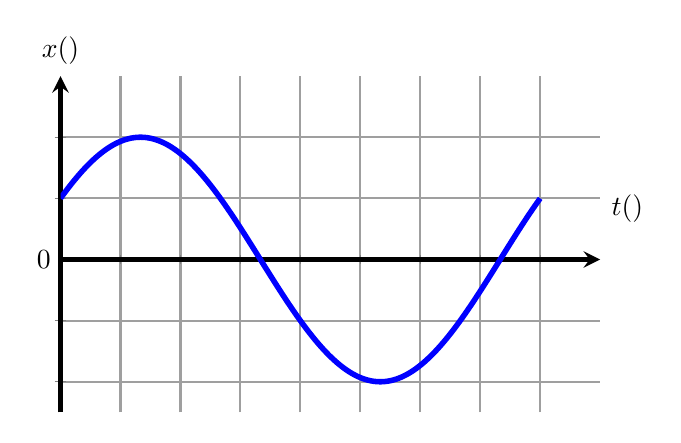
\begin{tikzpicture}  
		\begin{axis}[  ultra thick,yscale=0.75,
			xmin=0,  
			xmax=9,  
			xtick={0,1,...,8},
			ytick={-2,-1,...,2},
			minor x tick num=0,
			minor y tick num=0,
			ymin=-2.5,  
			ymax=3, 
			samples=300,
			yticklabels=\empty,
			xticklabels=\empty,
			axis lines=center, 
			grid style={step=1, line width =0.4pt, color=gray!40!white},
			grid=both, %giới hạn ô lưới
			major grid style={line width=0.8pt,gray!75!white},
			xlabel=$\xsi{t}{\left(\si{\second}\right)}$, 		ylabel=$\xsi{x}{\left(\si{\centi\meter}\right)}$,
			every axis y label/.style={at=(current axis.above origin),anchor=south},  
			every axis x label/.style={at=(current axis.right of origin),anchor=west},  ]
			\addplot [line width=2pt, blue, smooth, domain=0:8] {2*cos(deg(pi*x/4-pi/3))};  
			\coordinate (O) at (axis cs: 0,0);
		\end{axis}  
		\node[left] at (O) {0};
	\end{tikzpicture}
\end{center}	
	\choiceTF[t]
	{Tại thời điểm ban đầu, vật đi qua vị trí cân bằng theo chiều dương}
	{\True Pha dao động ban đầu của vật là $\xsi{-\dfrac{\pi}{3}}{\radian}$}
	{\True Nếu tỉ lệ trên trục $Ot$ là 1 ô tương ứng $\SI{0.1}{\second}$ thì chu kì dao động của vật là $\SI{0.8}{\second}$}
	{Nếu tỉ lệ trên trục $Ox$ là 1 ô tương ứng $\SI{4}{\centi\meter}$ thì biên độ dao động của vật là $\SI{16}{\centi\meter}$}
	\loigiai{}
\end{ex}
% ===================================================================
\begin{ex}
Đồ thị trong hình bên mô tả sự biến đổi gia tốc $a$ của một vật dao động điều hòa theo thời gian $t$. Lấy $\pi^2=10$.\\
\begin{center}
	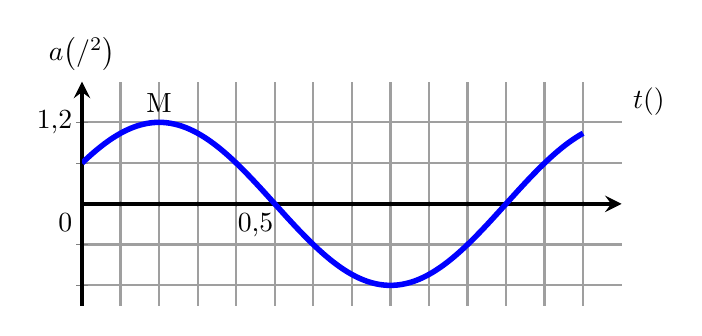
\begin{tikzpicture}  
		\begin{axis}[  ultra thick,yscale=0.5,
			xmin=0,  
			xmax=14,  
			xtick={0,1,...,13},
			ytick={-2,-1,...,2},
			minor x tick num=0,
			minor y tick num=0,
			ymin=-2.5,  
			ymax=3, 
			samples=300,
			yticklabels=\empty,
			xticklabels=\empty,
			axis lines=center, 
			grid style={step=1, line width =0.4pt, color=gray!40!white},
			grid=both, %giới hạn ô lưới
			major grid style={line width=0.8pt,gray!75!white},
			xlabel=$\xsi{t}{\left(\si{\second}\right)}$, 		ylabel=$\xsi{a}{\left(\si{\meter/\second^2}\right)}$,
			every axis y label/.style={at=(current axis.above origin),anchor=south},  
			every axis x label/.style={at=(current axis.right of origin),anchor=west},  ]
			\addplot [line width=2pt, blue, smooth, domain=0:13] {2*cos(deg(pi*x/6-pi/3))};  
			\coordinate (O) at (axis cs: 0,0);
			\coordinate (A) at (axis cs: 0,2);
			\coordinate (B) at (axis cs: 4.5,0);
				\coordinate (M) at (axis cs: 2,2);
		\end{axis}  
		\node[below left] at (O) {0};
		\node[left] at (A) {1,2};
		\node[below] at (B) {0,5};
		\node[above] at (M) {M};
	\end{tikzpicture}
\end{center}
Xét tính đúng/sai của các phát biểu sau:	
	\choiceTF[t]
	{\True Gia tốc cực đại của vật là $\SI{120}{\centi\meter/\second^2}$}
	{Chu kì dao động là $\SI{1.0}{\second}$}
	{Biên độ dao động là $\SI{5}{\centi\meter}$}
	{\True Li độ của vật khi có gia tốc tương ứng với điểm M trên đồ thị đang có giá trị âm}
	\loigiai{}
\end{ex}
\Closesolutionfile{ans}
\section{Câu trắc nghiệm trả lời ngắn} \textit{Thí sinh trả lời từ câu 1 đến câu 6}
\setcounter{ex}{0}
\Opensolutionfile{ans}[ans/G11-5-TL]
% ===============================================================
\begin{ex}
	Một chiếc xe máy chạy trên một con đường lát gạch, cứ cách khoảng $\SI{4}{\meter}$ trên đường lại có một cái rãnh nhỏ. Chu kì dao động riêng của khung xe máy trên các lò xo giảm xóc là $\SI{0.5}{\second}$. Xe bị xóc mạnh nhất khi chuyển động với tốc độ bằng bao nhiêu $\si{\meter/\second}$?
	\shortans{8}
	\loigiai{
		Xe bị xóc mạnh nhất khi chu kì ngoại lực kích thích bằng chu kì dao động riêng của khung xe $T=T_0=\SI{4}{\second}$.\\
		Tốc độ của xe khi xe xóc mạnh nhất:
		$$v=\dfrac{s}{T}=\SI{8}{\meter/\second}.$$
	}
\end{ex}
% ===============================================================
\begin{ex}
Một con lắc lò xo đang dao động tắt dần với cơ năng ban đầu của nó là $\SI{10}{\joule}$, sau ba chu kì dao động biên độ của nó giảm $\SI{10}{\percent}$. Phần cơ năng chuyển hoá thành nhiệt sau khoảng thời gian đó bằng bao nhiêu joule ($\si{\joule}$)?	
	\shortans{1,9}
	\loigiai{
		Gọi $A$ là biên độ dao động ban đầu của vật nặng, cơ năng ban đầu của vật
		$$W=\dfrac{1}{2}kA^2=\SI{10}{\joule}$$
		Sau 3 chu kì dao động $A'=0,9A$
		$$\Rightarrow W'=\dfrac{1}{2}kA'^2=0,81\cdot\dfrac{1}{2}kA^2=\SI{8.1}{\joule}$$
		Phần cơ năng chuyển hoá thành nhiệt:
		$$\Delta W=W-W'=\SI{1.9}{\joule}.$$
	}
\end{ex}
% ===============================================================
\begin{ex}
	Cho đồ thị vận tốc theo thời gian của một vật dao động điều hòa như hình vẽ. Biết rằng khối lượng của vật là $\SI{150}{\gram}$. Lấy $\pi^2=10$.
	\begin{center}
		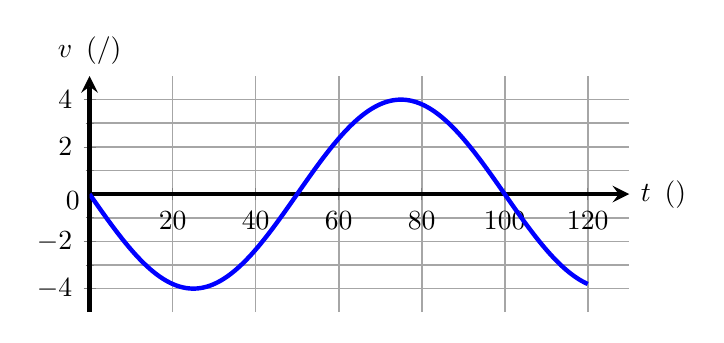
\begin{tikzpicture}  
			\begin{axis}[  ultra thick,
				xmin=0,  
				xmax=130,  
				xtick={0,20,40,60,...,120},
				ytick={-4,-2,0,2,4},
				minor x tick num=0,
				minor y tick num=1,
				ymin=-5,  
				ymax=5, 
				y=0.3cm,
				samples=300,
				axis lines=center, 
				grid style={step=1, color=gray!70!white, line width=0.6pt},
				grid=both,
				xlabel=$t\ \left(\si{\milli\second}\right)$, 
				ylabel=$v\ \left(\si{\meter/\second}\right)$, 
				every axis y label/.style={at=(current axis.above origin),anchor=south},  
				every axis x label/.style={at=(current axis.right of origin),anchor=west},  ]
				\addplot [ultra thick, blue, smooth, domain=0:120] {4*cos(deg(0.02*pi*x+pi/2))}; 
			\end{axis}  
			\node[label={[left]90:0}] at (0,1.3){};
		\end{tikzpicture}
	\end{center}
	Hãy xác định gia tốc của vật tại thời điểm $\SI{100}{\milli\second}$ theo đơn vị $\si{\meter/\second^2}$. \textit{(Kết quả làm tròn đến phnguyên)}.
	\shortans{253 }
	\loigiai{
		Chu kì dao động của vật:
		$$T=\SI{100}{\milli\second}$$
		Tần số góc dao động:
		$$\omega=\dfrac{2\pi}{T}=\xsi{20\pi}{\radian/\second}$$
		Biên độ dao động của vật:
		$$A=\dfrac{v_\text{max}}{\omega}=\dfrac{\SI{4E2}{\centi\meter/\second}}{\xsi{20\pi}{\radian/\second}}\approx\xsi{2\sqrt{10}}{\centi\meter}$$
		Tại thời điểm $t=\SI{100}{\milli\second}$ vật có vận tốc bằng 0 và đang giảm $\Rightarrow$ vật ở vị trí biên dương $x=A=\SI{6.37}{\centi\meter}$.\\
		Gia tốc của vật lúc này:
		$$a=-\omega^2 x=-\left(\xsi{20\pi}{\radian/\second}\right)^2\cdot\left(\xsi{2\sqrt{10}\cdot10^{-2}}{\meter}\right)\approx\SI{252.98}{\meter/\second^2}.$$
	}
\end{ex}
% ===============================================================
\begin{ex}
Một lò xo có khối lượng không đáng kể bị kéo dãn $\SI{3.0}{\centi\meter}$ nếu chịu tác dụng của lực có độ lớn $\SI{7.5}{\newton}$ tác dụng dọc theo trục lò xo. Vật nhỏ khối lượng $\SI{0.5}{\kilogram}$ nằm trên mặt phẳng nằm ngang không ma sát và được gắn vào đầu tự do của lò xo. Người ta kéo vật nặng đến vị trí lò xo dãn $\SI{5}{\centi\meter}$ rồi thả nhẹ cho vật dao động. Xác định vận tốc của vật tại thời điểm $t=\SI{0.5}{\second}$ theo đơn vị $\si{\centi\meter/\second}$. \textit{(Kết quả làm tròn đến phần nguyên)}.
	\shortans{110}
	\loigiai{
		Độ cứng của lò xo:
		$$k=\dfrac{F}{\Delta\ell}=\dfrac{\SI{7.5}{\newton}}{\SI{3E-2}{\centi\meter}}=\SI{250}{\newton\meter}.$$
	Tần số góc dao động của vật:
		$$\omega=\sqrt{\dfrac{k}{m}}=\sqrt{\dfrac{\SI{250}{\newton/\meter}}{\SI{0.5}{\kilogram}}}=\xsi{10\sqrt{5}}{\radian/\second}.$$
	Chọn gốc thời gian lúc thả vật, chiều dương cùng chiều biến dạng ban đầu của lò xo.\\
		Phương trình dao động của vật:
		$$x=A\cos\left(\omega t+\varphi_0\right)=\xsi{5\cos\left(10\sqrt{5}t\right)}{\centi\meter}$$
	Phương trình vận tốc của vật:
		$$v=-\omega A\sin\left(\omega t+\varphi_0\right)=\xsi{-50\sqrt{5}\sin\left(10\sqrt{5}t\right)}{\centi\meter/\second}$$
		Tại thời điểm $t=\SI{0.5}{\second}$ thì $v\approx\SI{109.9}{\centi\meter/\second}.$
	}
\end{ex}
% ===============================================================
\begin{ex}
	Đồ thị hình bên mô tả sự thay đổi động năng theo li độ của của quả cầu có khối lượng $\SI{0.1}{\kilogram}$ trong một con lắc lò xo treo thẳng đứng.
	\begin{center}
		\includegraphics[width=0.35\linewidth]{../figs/D11-005-1}
	\end{center}
	Thế năng của quả cầu khi ở vị trí có li độ $\SI{2}{\centi\meter}$ là bao nhiêu milli joule $\left(\si{\milli\joule}\right)$? \textit{(Kết quả làm tròn đến 1 chữ số sau dấu phẩy thập phân)}.
	\shortans{53,3}
	\loigiai{
		Từ đồ thị ta có $W_{\text{đ max}}=\dfrac{1}{2}mv^2_{\text{max}}=\SI{0.12}{\joule}\Rightarrow v_{\text{max}}=\xsi{\dfrac{2\sqrt{15}}{5}}{\meter/\second}$.\\
		Tần số góc dao động:
		$$\omega=\dfrac{v_{\text{max}}}{A}=\dfrac{\dfrac{2\sqrt{15}}{5}}{0,03}=\xsi{\dfrac{40\sqrt{15}}{3}}{\radian/\second}.$$
		Thế năng của con lắc khi quả cầu ở vị trí có li độ $\SI{2}{\centi\meter}$:
		$$W_t=\dfrac{1}{2}m\omega^2x^2=\dfrac{1}{2}\cdot0,1\cdot\left(\dfrac{40\sqrt{15}}{3}\right)^2\cdot\left(0,02\right)^2\approx\SI{53.3}{\milli\joule}.$$
	}
\end{ex}
% ===============================================================
\begin{ex}
	Quả lắc của đồng hồ cổ treo tường có tác dụng vận hành cho đồng hồ chạy đúng giờ.\\
	\immini{
		Cứ sau mỗi chu kì dao động của quả lắc, do sức cản và việc vận hành hệ thống bánh răng để các kim đồng hồ chạy nên nó tiêu hao năng lượng $\Delta E=\SI{0.100}{\milli\joule}$. Năng lượng này được lấy từ một quả tạ có trọng lượng $P=\SI{50.0}{\newton}$ treo trong hoặc ngoài đồng hồ. Nếu chạy trong thời gian $t=10\ \text{ngày}$ thì quả tạ sẽ giảm độ cao bao nhiêu mét? Biết trong 30 chu kì dao động của quả lắc thì kim giây chuyển động được một vòng. \textit{(Kết quả làm tròn đến 2 chữ số sau dấu phẩy thập phân)}.}
		{
		\includegraphics[width=0.5\linewidth]{../figs/D11-2-2}
		}
	\shortans{0,86}
	\loigiai{
		Mỗi phút, kim giây chuyển động hết 1 vòng và con lắc đồng hồ thực hiện 30 chu kì.\\
		Như vậy, số chu kì con lắc thực hiện được trong 10 ngày là:
		$$N=10 \cdot24\cdot\left(\SI{60}{\minute}\right)\cdot\left(30\ \text{chu kì/\si{\minute}}\right)=432000\ \text{chu kì}$$
		Tổng năng lượng tiêu hao trong 10 ngày:
		$$E=\left(432000\ \text{chu kì}\right)\cdot\left(\SI{0.100E-3}{\joule/\text{chu kì}}\right)=\SI{43.2}{\joule}$$
		Năng lượng tiêu hao này được bù bằng độ giảm thế năng trọng trường của quả tạ. Do đó, độ cao quả tạ bị giảm một đoạn:
		$$\Delta h=\dfrac{E}{P}=\dfrac{\SI{43.2}{\joule}}{\SI{50.0}{\newton}}=\SI{0.864}{\meter}.$$
	}
\end{ex}
\Closesolutionfile{ans}
\begin{center}
	\textbf{--- HẾT ---}
\end{center}